\chapter{Teamvorstellung}
\setauthor{Raffeiner Christine, Weissengruber Nina}
\subsection{Team}
\subsubsection{Raffeiner Christine}
\begin{wrapfigure}{r}{0.3\textwidth}
    \begin{center}
      \includegraphics[width=0.3\textwidth]{pics/Chrissy.jpg}
    \end{center}
\end{wrapfigure}
Christine Raffeiner ist eine 20 Jahre junge Musterschülerin, die viel Zeit und Mühe investiert um ihre 
schulischen Ziele zu erreichen. Sie ist bereits das sechste Jahr an der HTL Leonding, jedoch ist sie in 
allen Fächern eine der Besten aus ihrer Klasse und ist auch gerne bereit anderen zu helfen und ihnen 
Fragen zu erklären. Zusätzlich zu ihrer Hilfsbereitschaft strahlt sie Fröhlichkeit aus und ist eine Person 
mit der man gern über alle möglichen Themen spricht, egal ob schulischer oder privater Natur.
\newline
\subsubsection{Weissengruber Nina}
\begin{wrapfigure}{r}{0.3\textwidth}
    \begin{center}
      \includegraphics[width=0.3\textwidth]{pics/nina.jpg}
    \end{center}
\end{wrapfigure}
Nina Weissengruber die perfekte Ergänzung für jedes Team und ein richtiges Energiepacket, die die 
Aufmerksamkeit auf sich zieht.  
Nina ist eine hervorragende Schülerin, die man sich zum 
Vorbild nehmen kann und muss, denn sie schafft es ohne große Hindernisse, zu bestehen. Besonders erwähnenswert sind auch 
ihre ausgezeichneten Kenntnisse in Mathematik und Apex.

\subsubsection{Über Uns}
Zusammenfassend ist noch zu sagen, dass wir ausgezeichnet zusammenarbeiten konnten, obwohl wir uns vor unserem Projekt  nicht wirklich gut kannten. 
Unsere Arbeitsweise betrachtend spielten wir gut zusammen 
und verfolgten ohne viel Absprache die selben Ziele.

\chapter{Wichtige Lektionen}
\setauthor{Raffeiner Christine, Weissengruber Nina}
Die offensichtlichste Lektion die wir gelernt haben, war die Handhabung von längerfristigen Projekten, die 
hohe Priorität und gewisse Eigenverantwortung mit sich ziehen. Um das noch weiter zu führen wurden auch die 
Erfahrungen gemacht, die Projektarbeit völlig außerhalb der Schulstunden neben Schul- und Lernstress mit sich 
bringen. Dazu zählen besonders das Einteilen von Aufgaben und Zeitmanagement. Persönliche Erfahrungen wurden 
besonders im Bereich der Testimplementierung und Wichtigkeit dieser erzielt. Auch wurde außerhalb der 
bereits erlernten Kenntnisse wissen im Bereich des Keycloak und Reverse-Proxy gesammelt. Rückschließend sind 
wir zu dem Entschluss gekommen, dass die stressfreie Zeit während der Sommerferien besser hätten nutzen sollen.

\chapter{Protokolle}
\setauthor{Raffeiner Christine}
Folgend befinden sich sämtliche Gesprächsprotokolle der Meetings, die das Team im Laufe 
der Arbeit mit ihrem Betreuer Herrn Professor Thomas Stütz geführt hat. 
\newline
Die Protokolle stellen eine Zusammenfassung der jeweiligen Meetings dar. \cite{noauthor_asciidock_nodate}

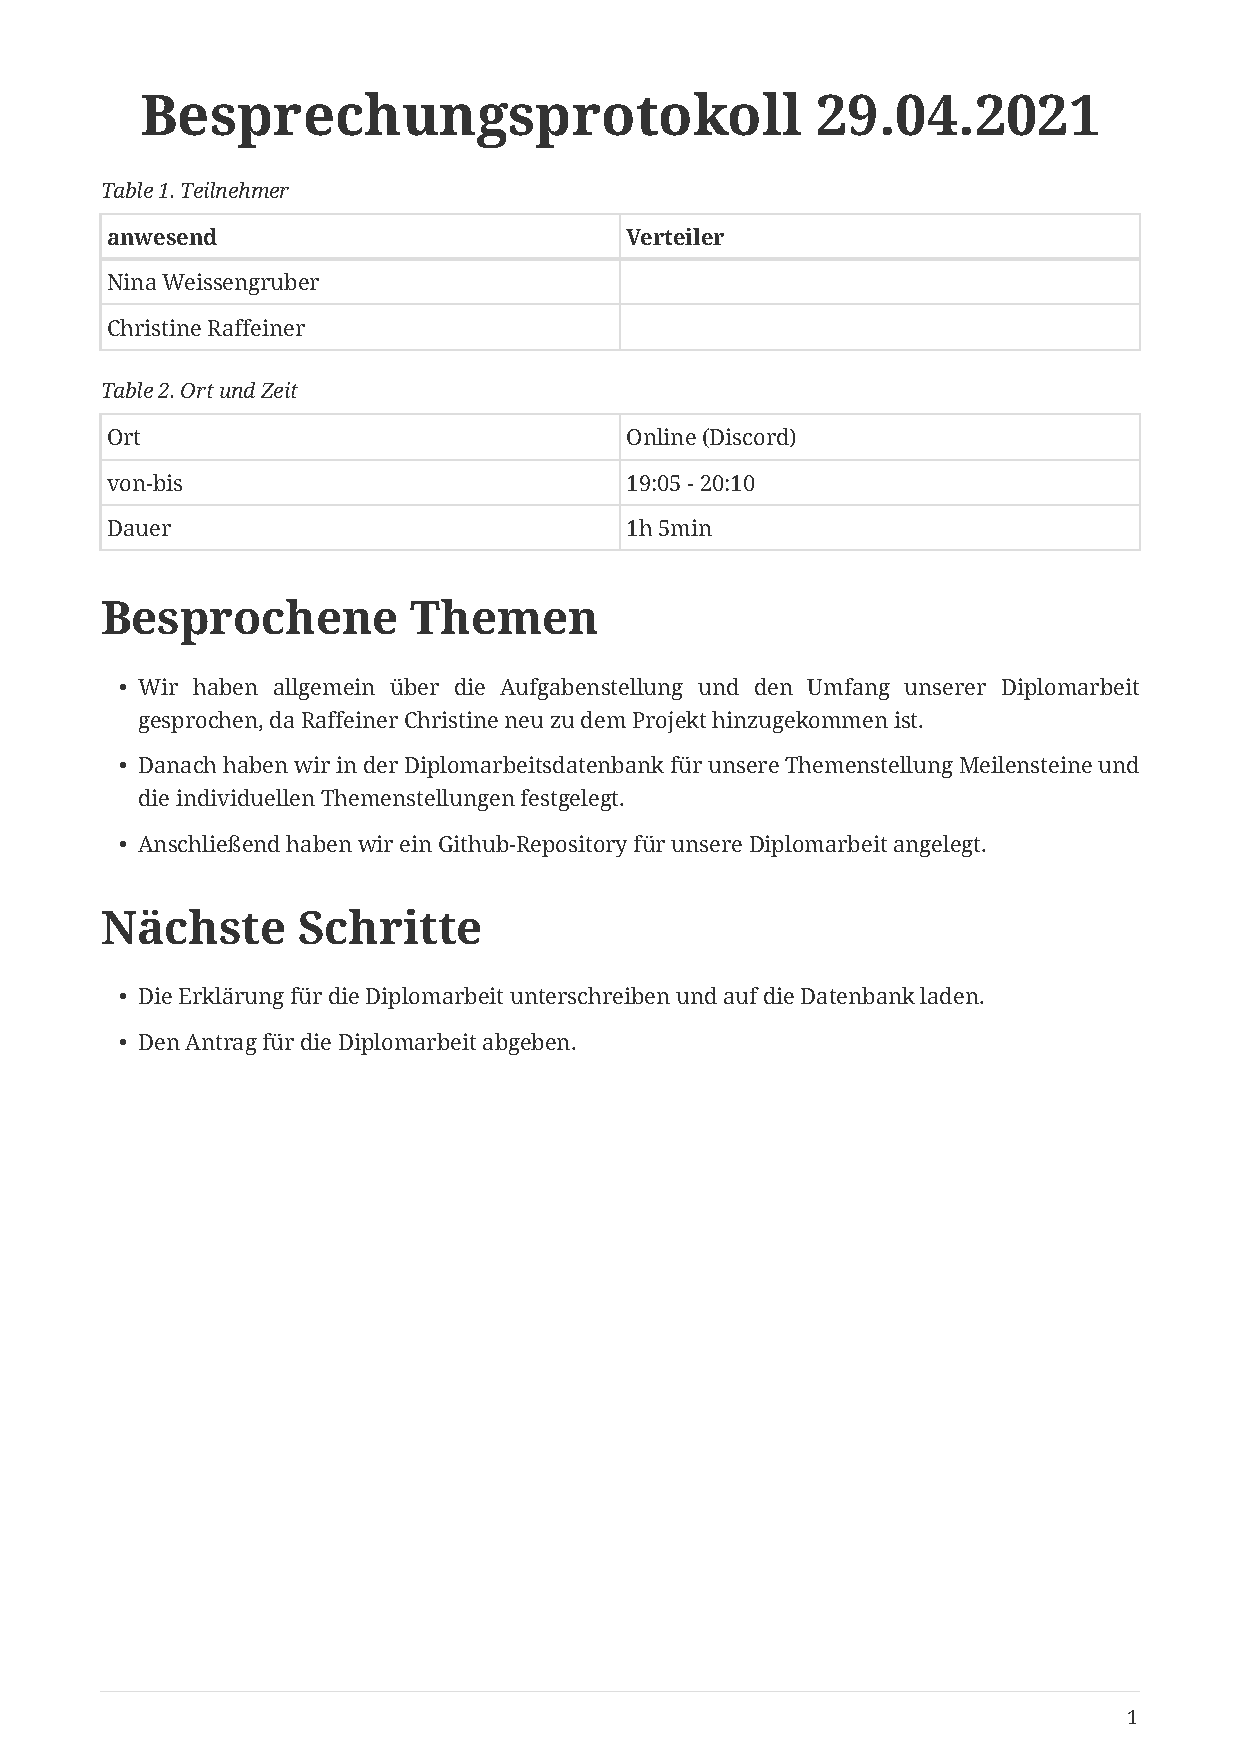
\includepdf{./protocols/meeting_29.04.2021}

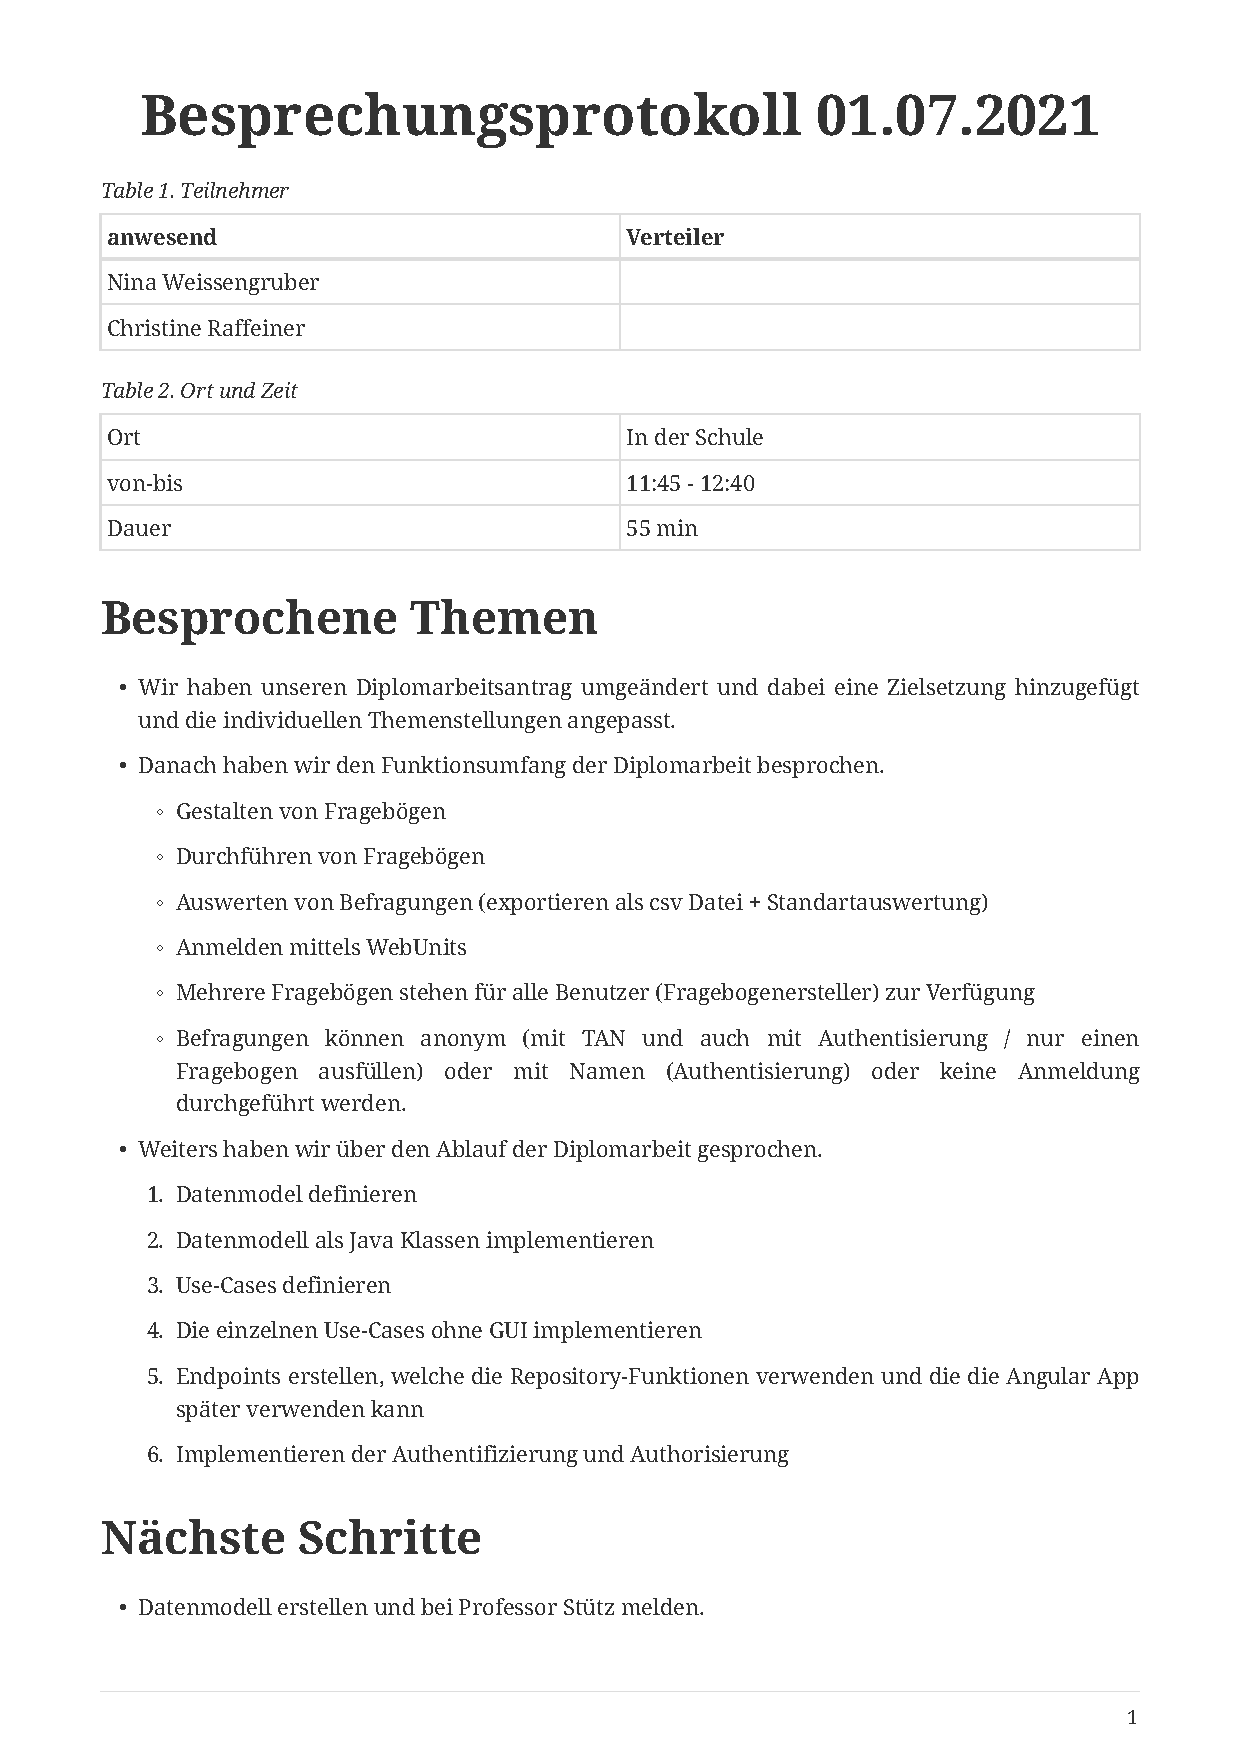
\includepdf{./protocols/meeting_01.07.2021}

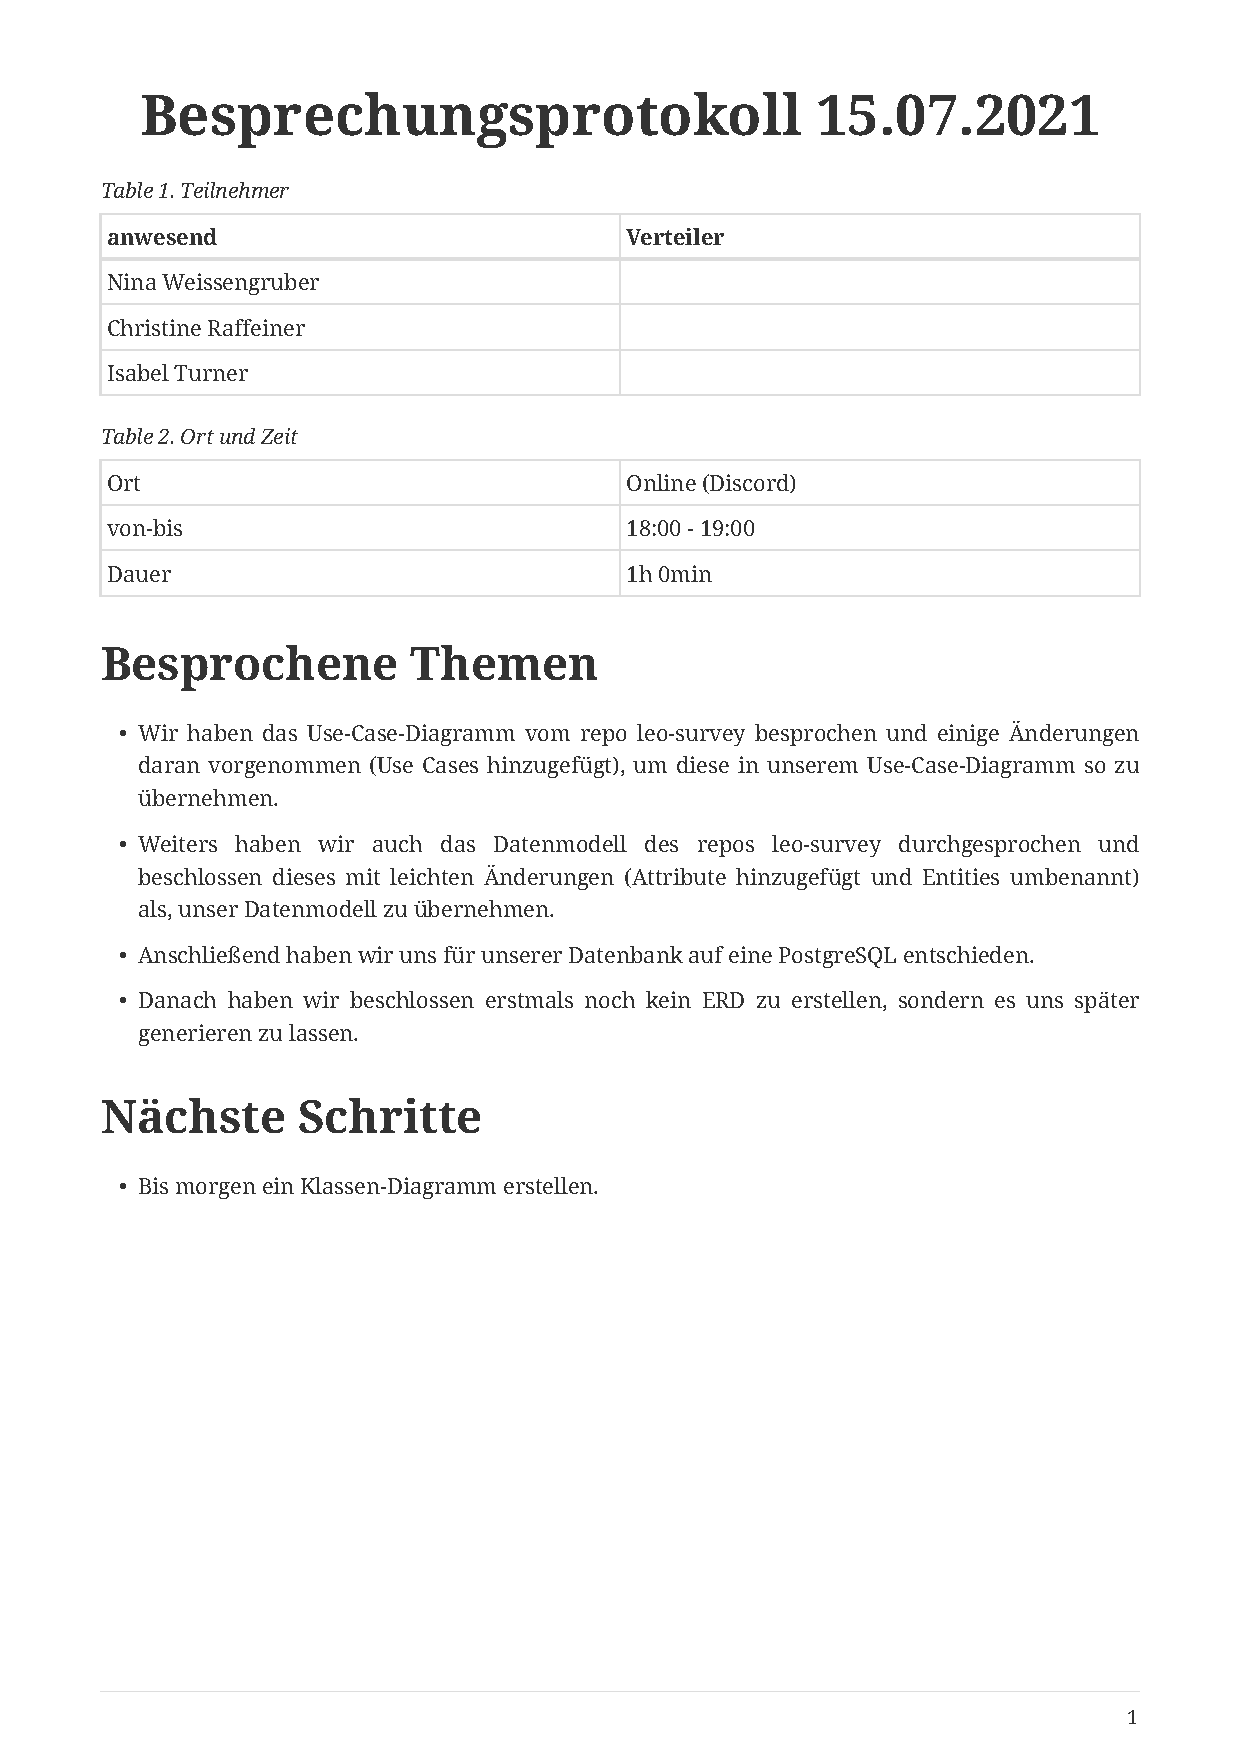
\includepdf{./protocols/meeting_15.07.2021}

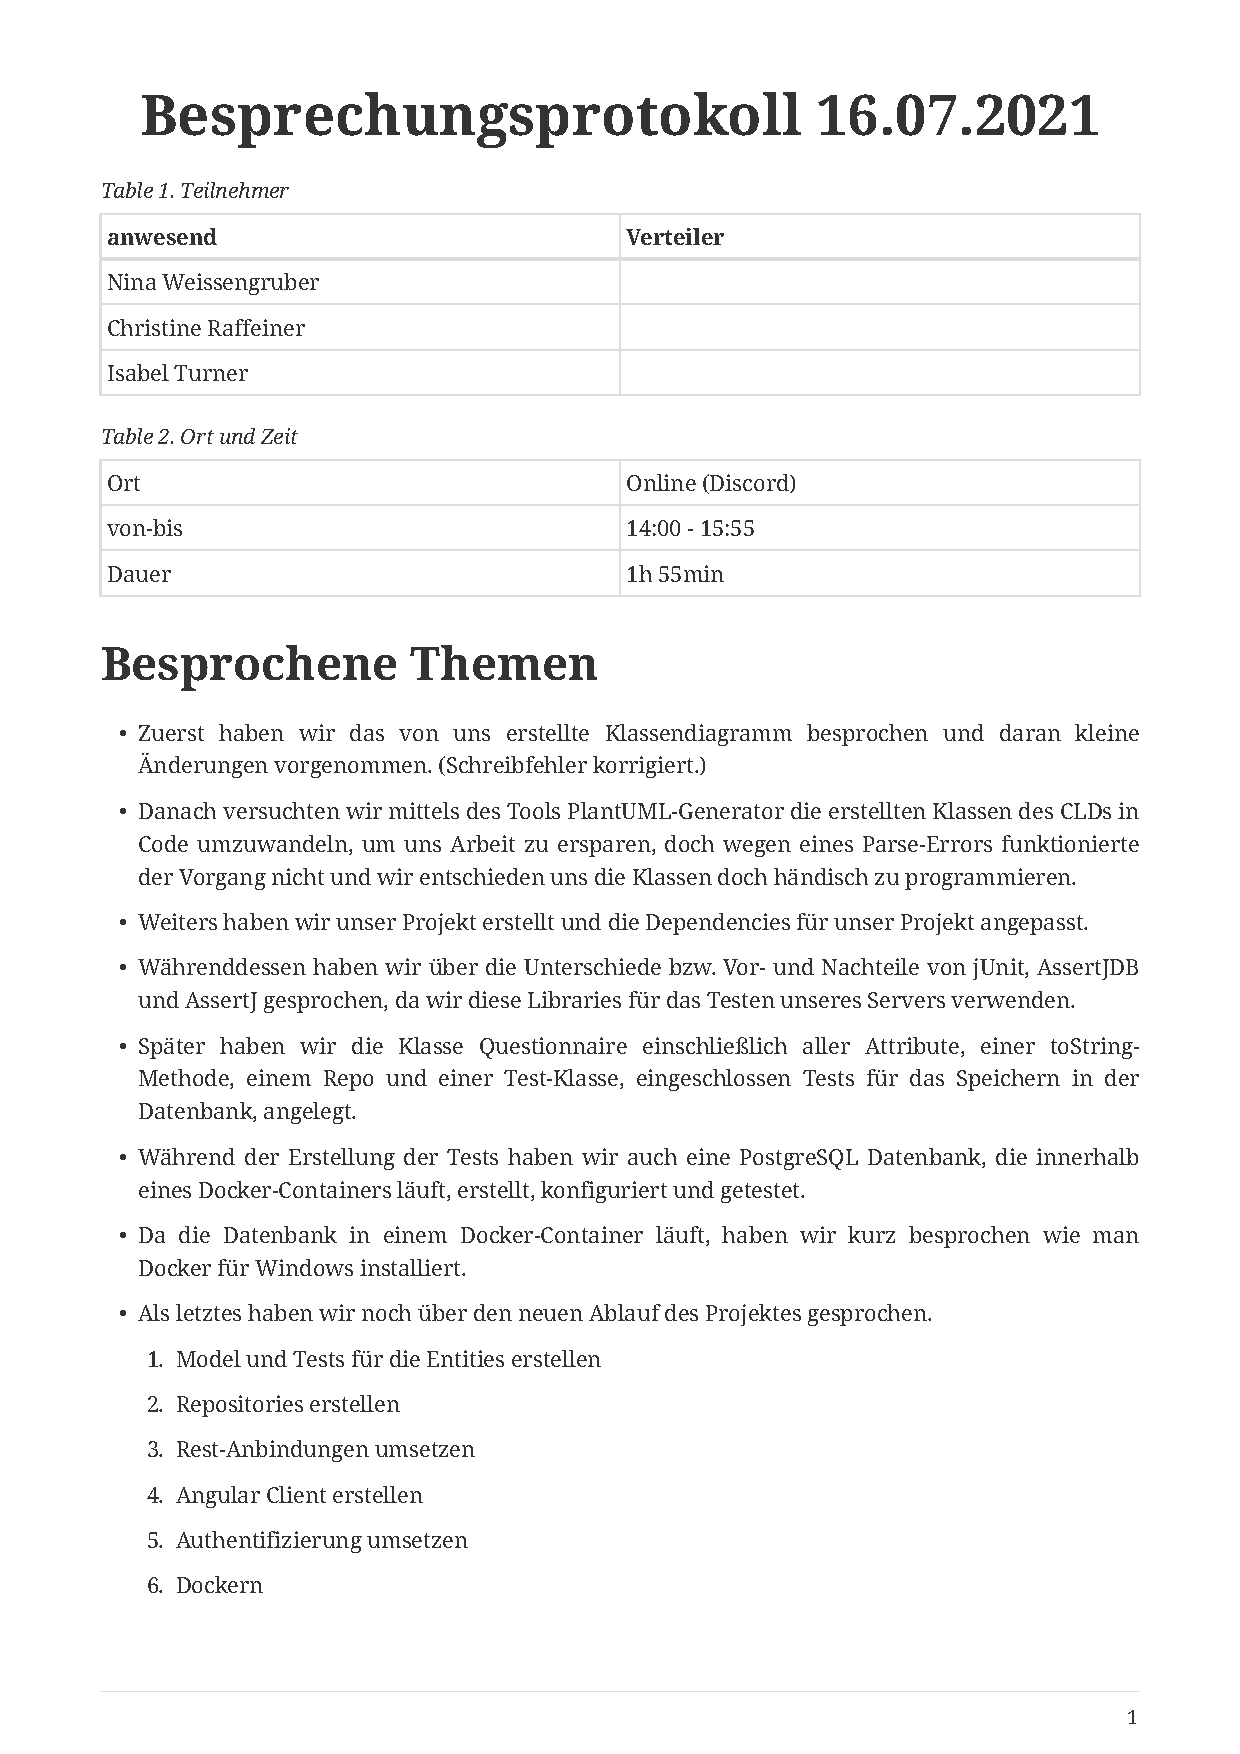
\includepdf{./protocols/meeting_16.07.2021}
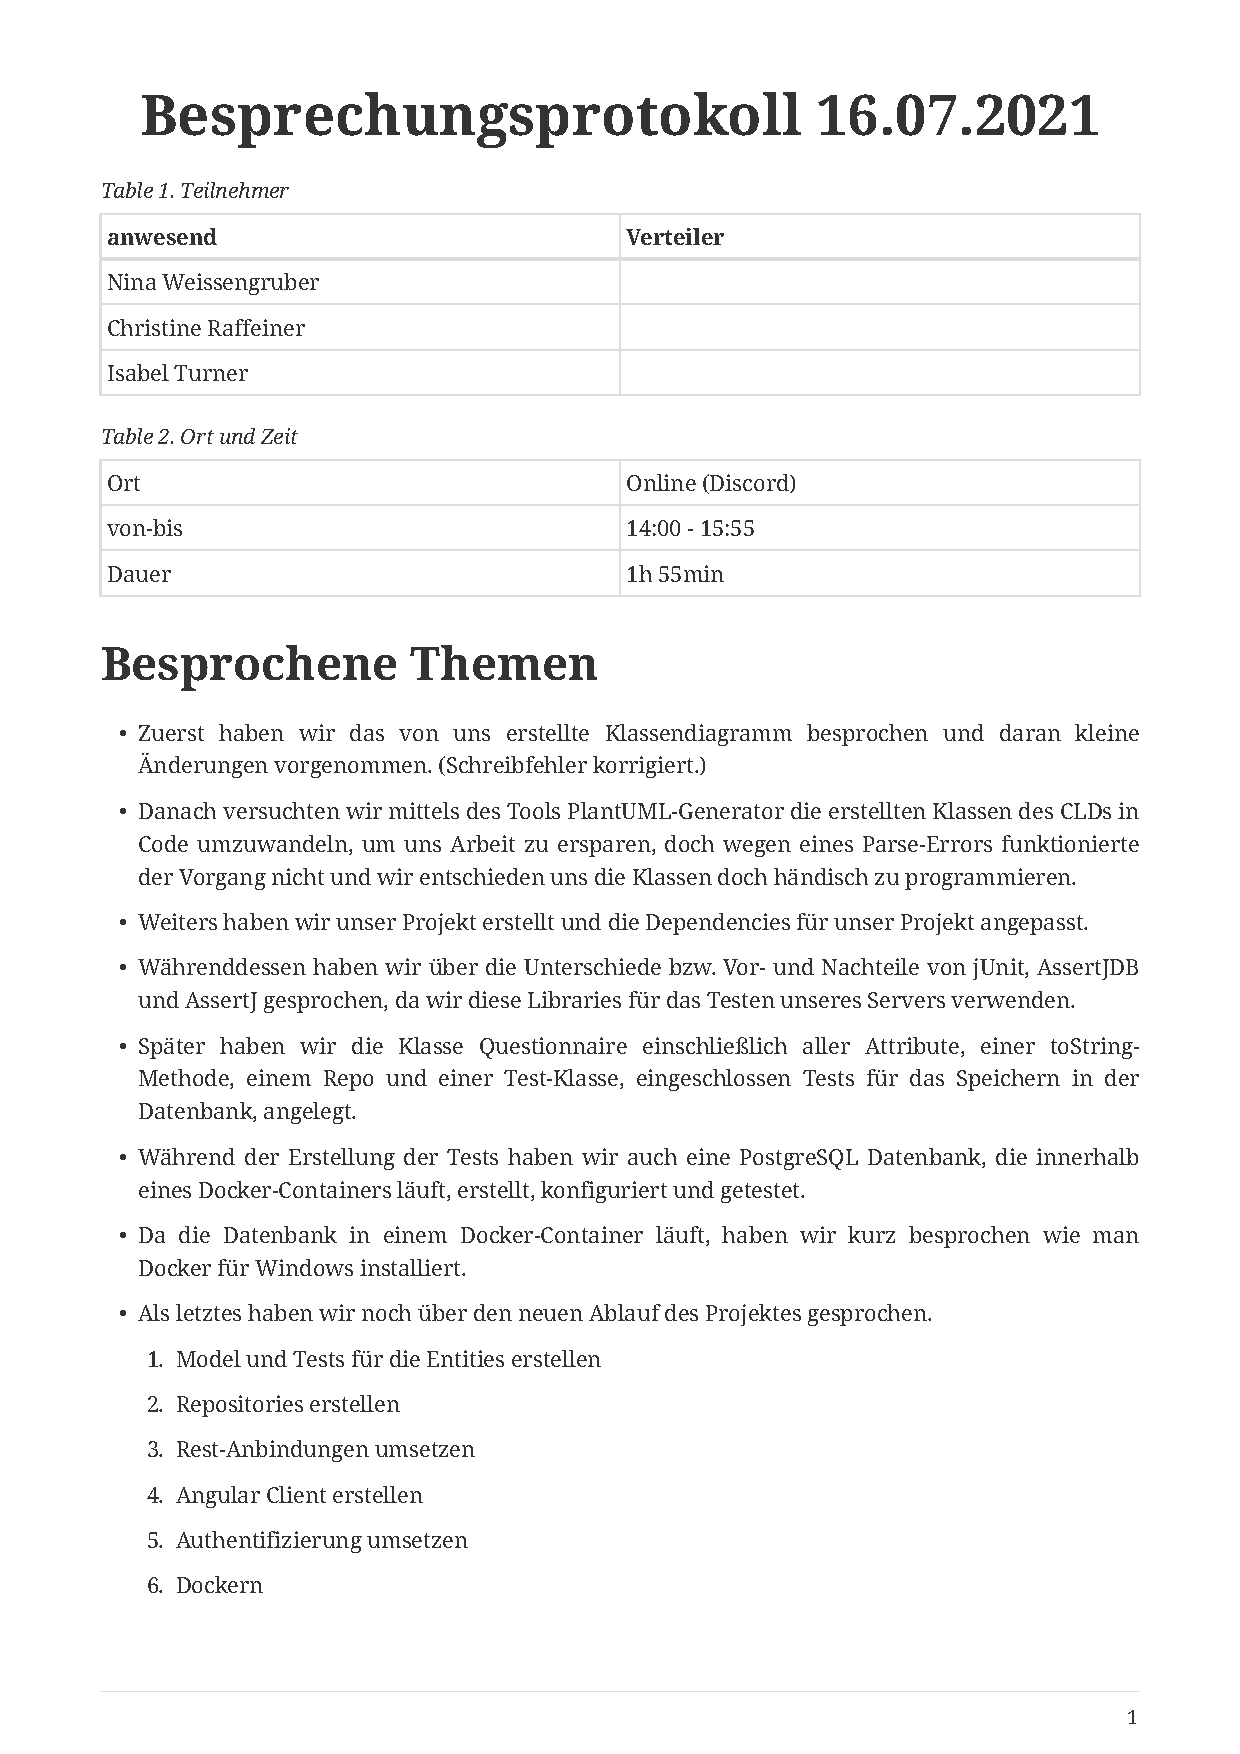
\includepdf[page=2]{./protocols/meeting_16.07.2021}

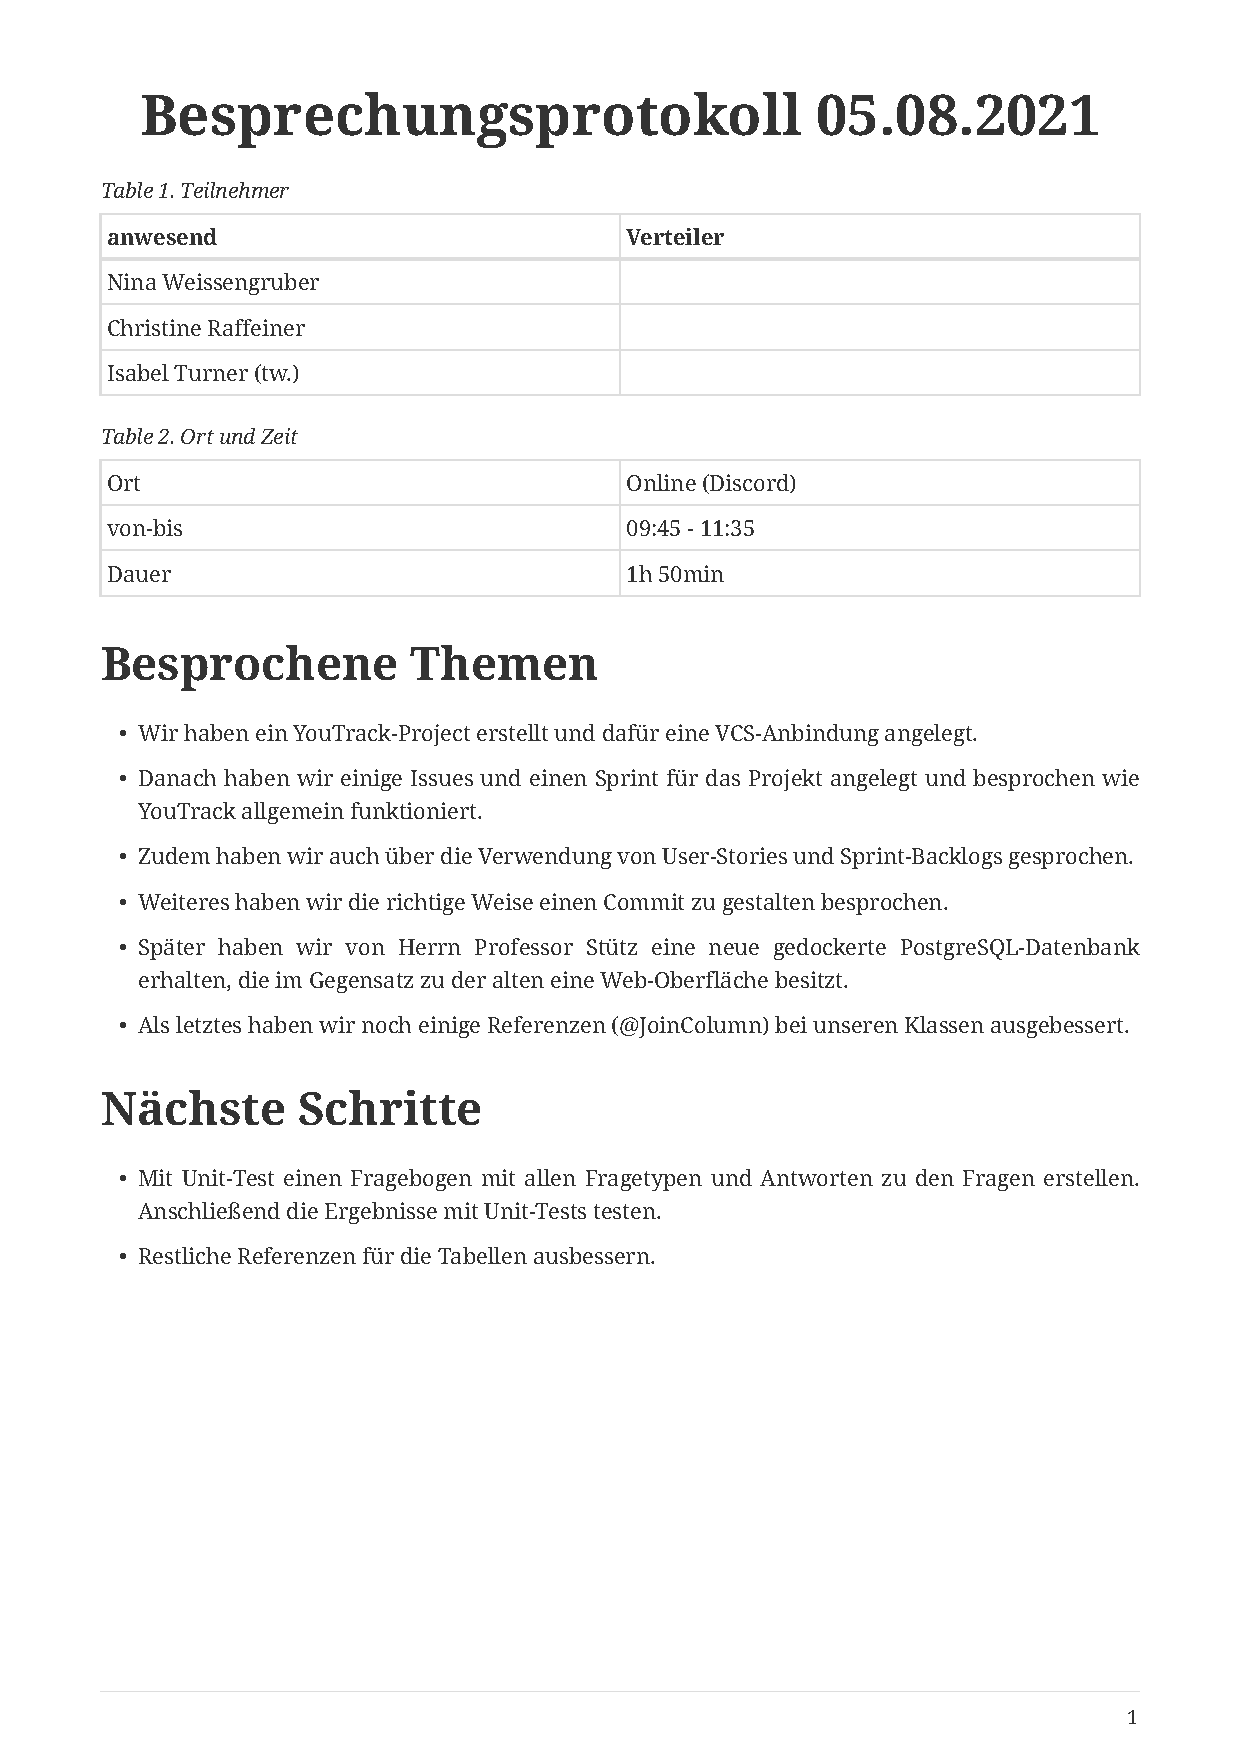
\includepdf{./protocols/meeting_05.08.2021}

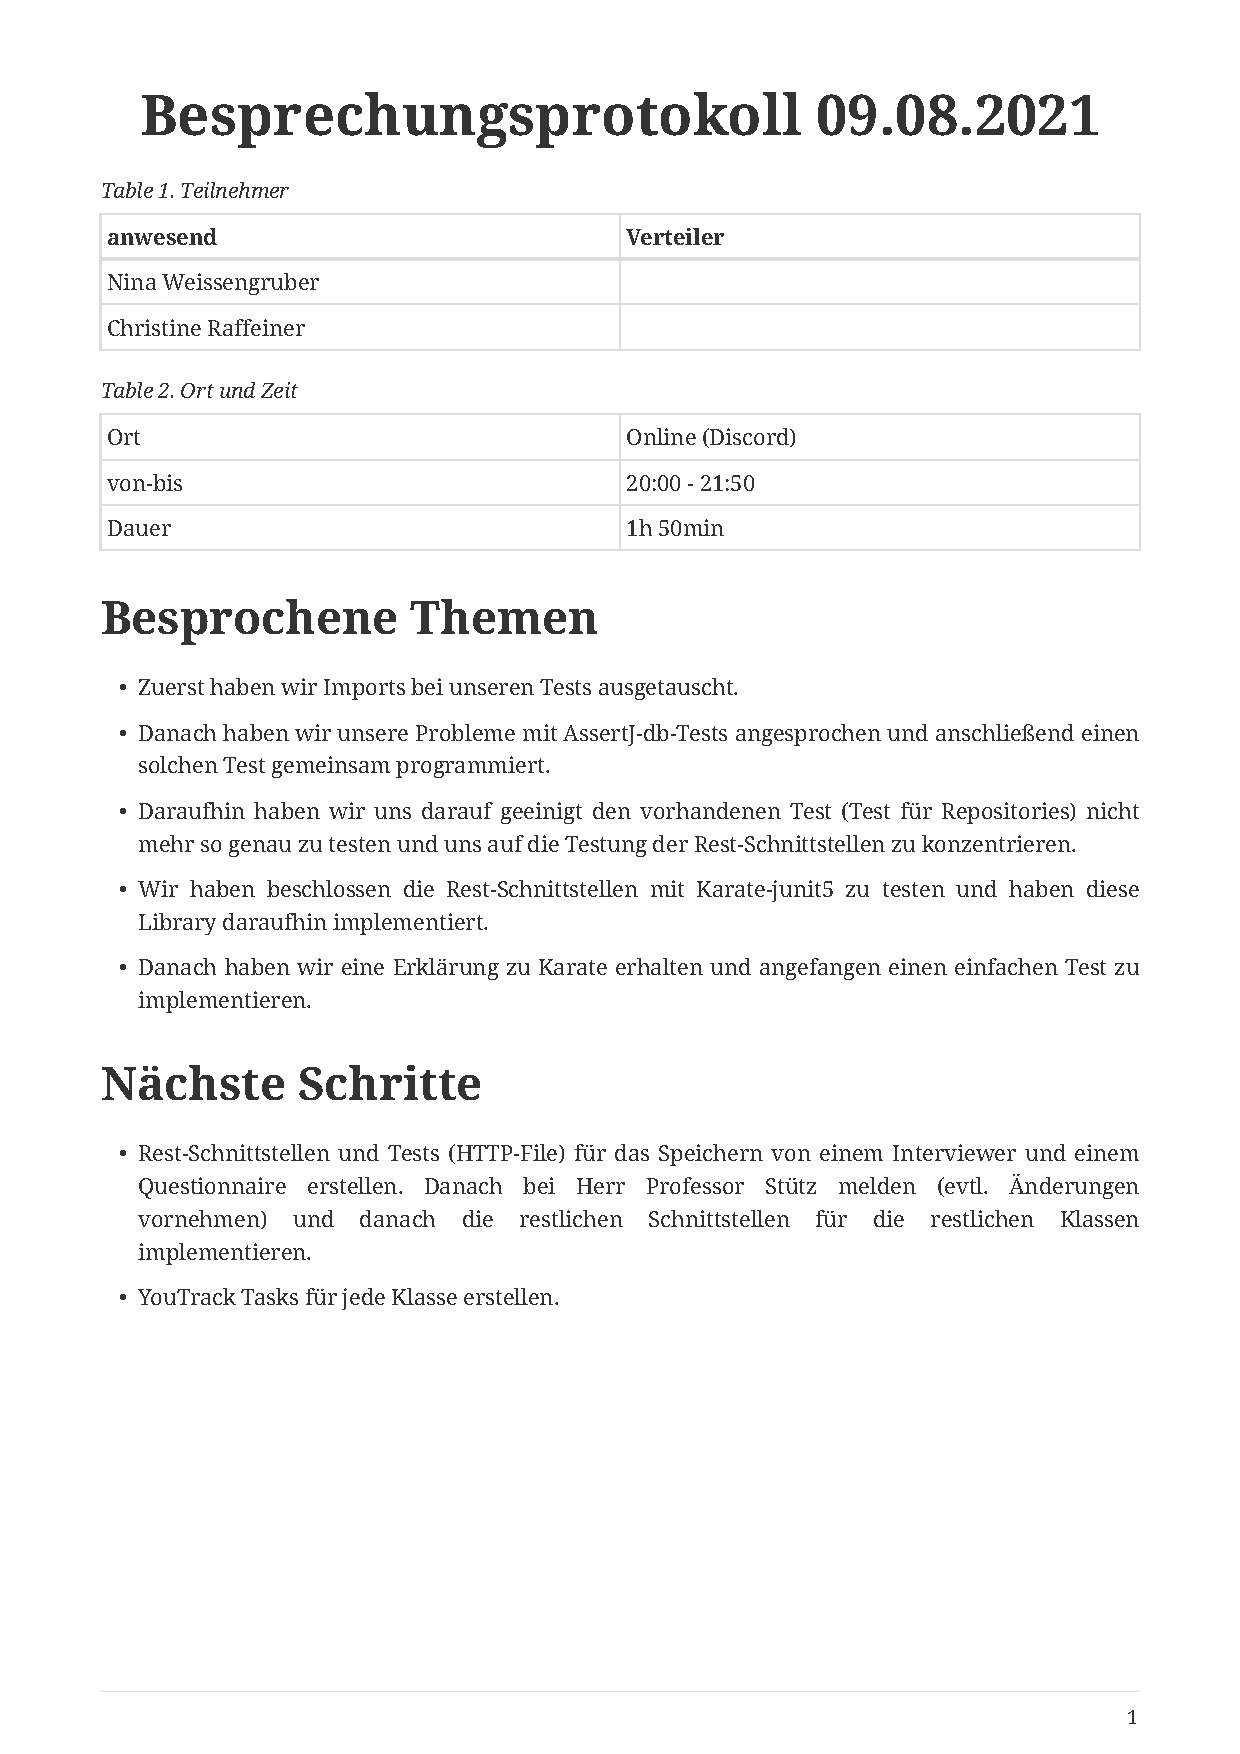
\includepdf{./protocols/meeting_09.08.2021}

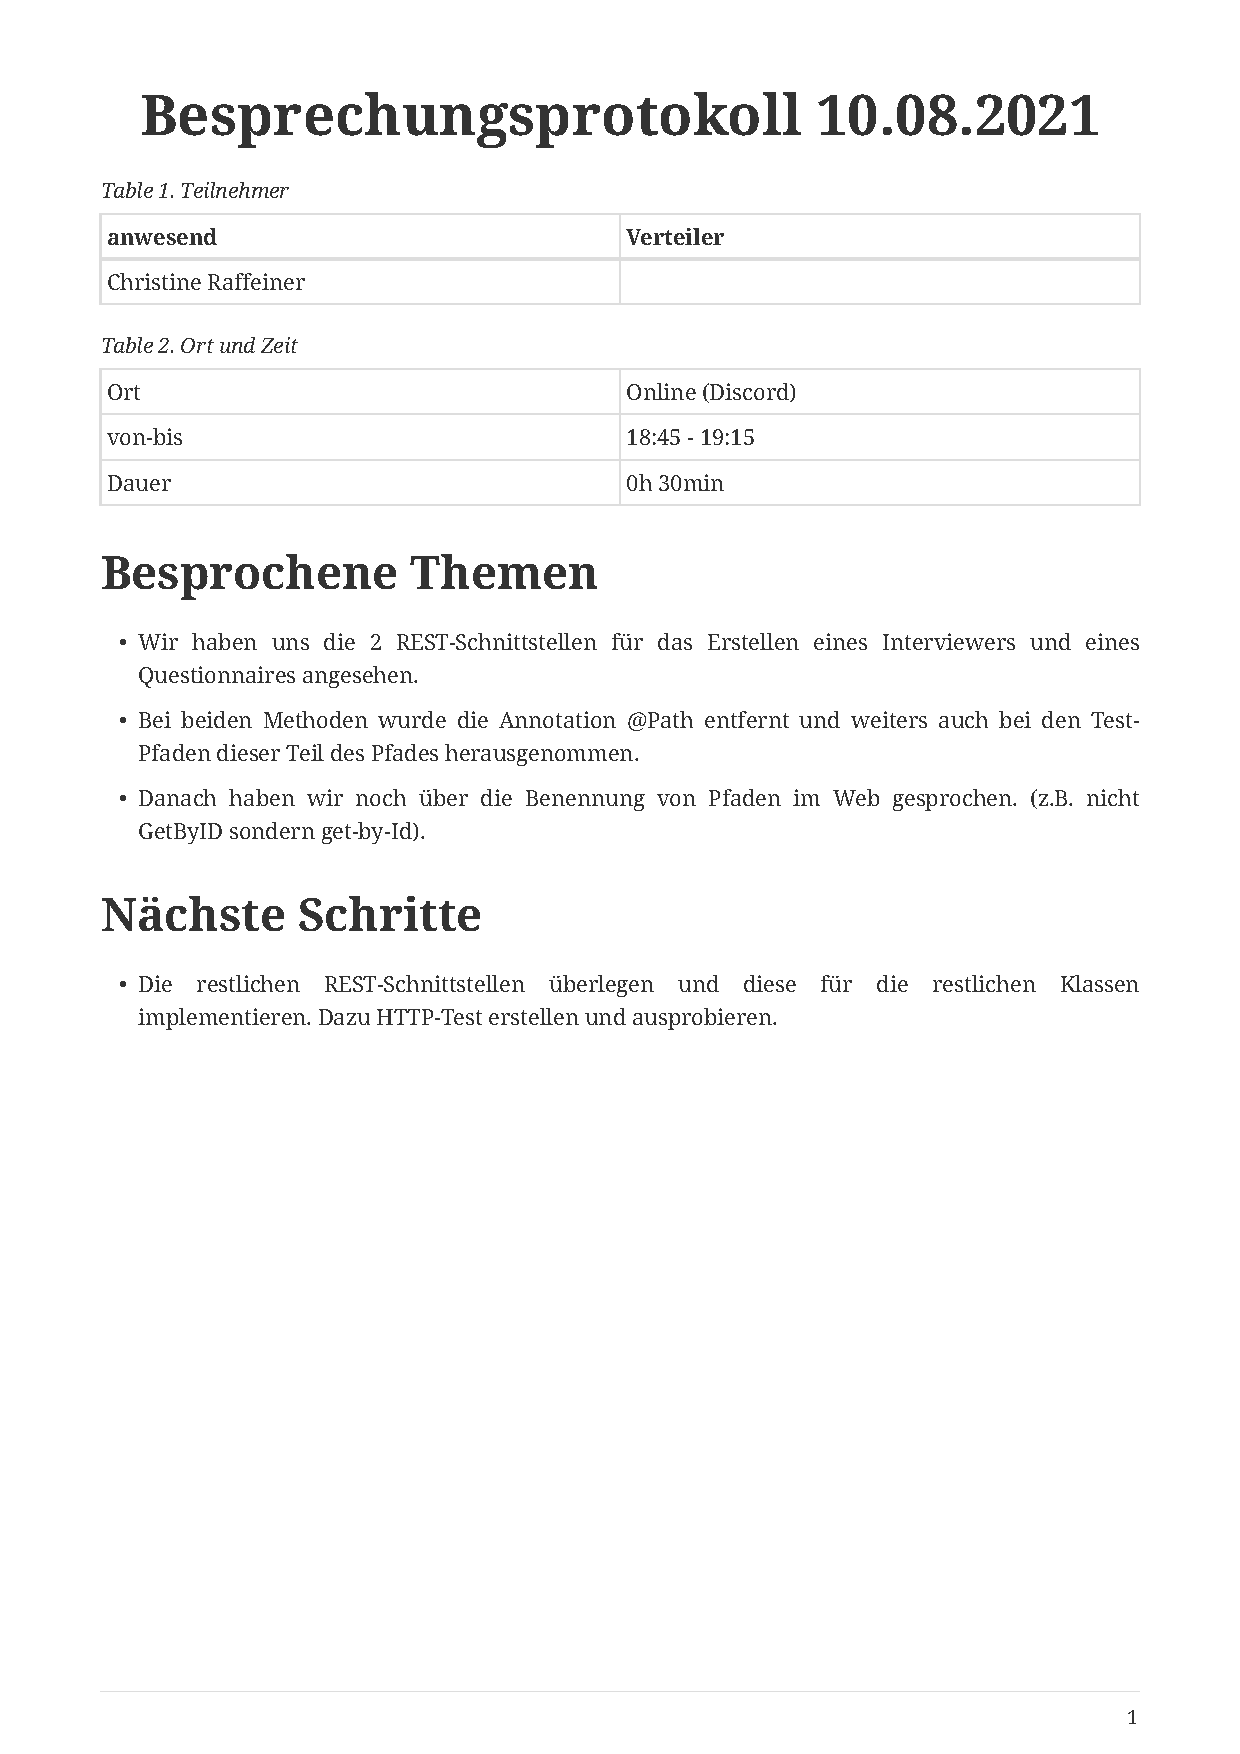
\includepdf{./protocols/meeting_10.08.2021}

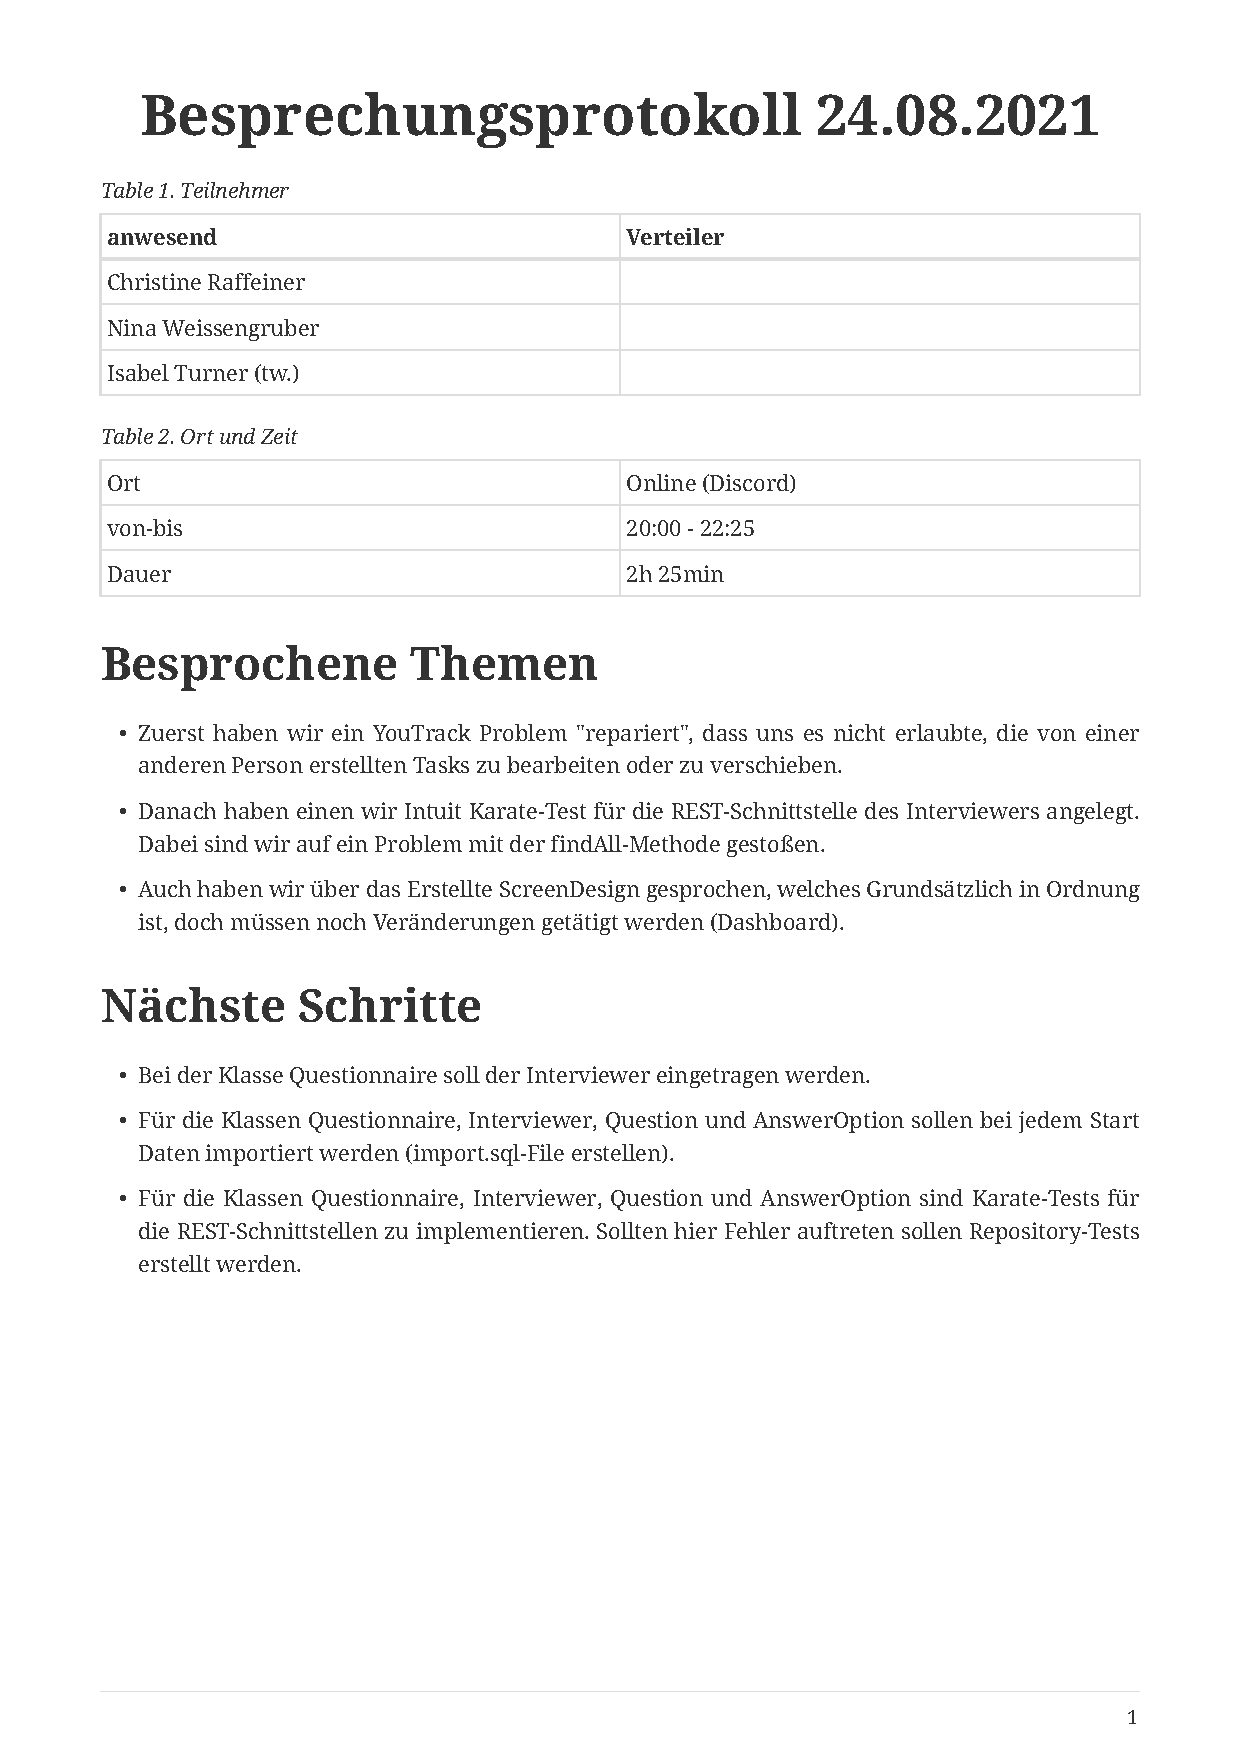
\includepdf{./protocols/meeting_24.08.2021}

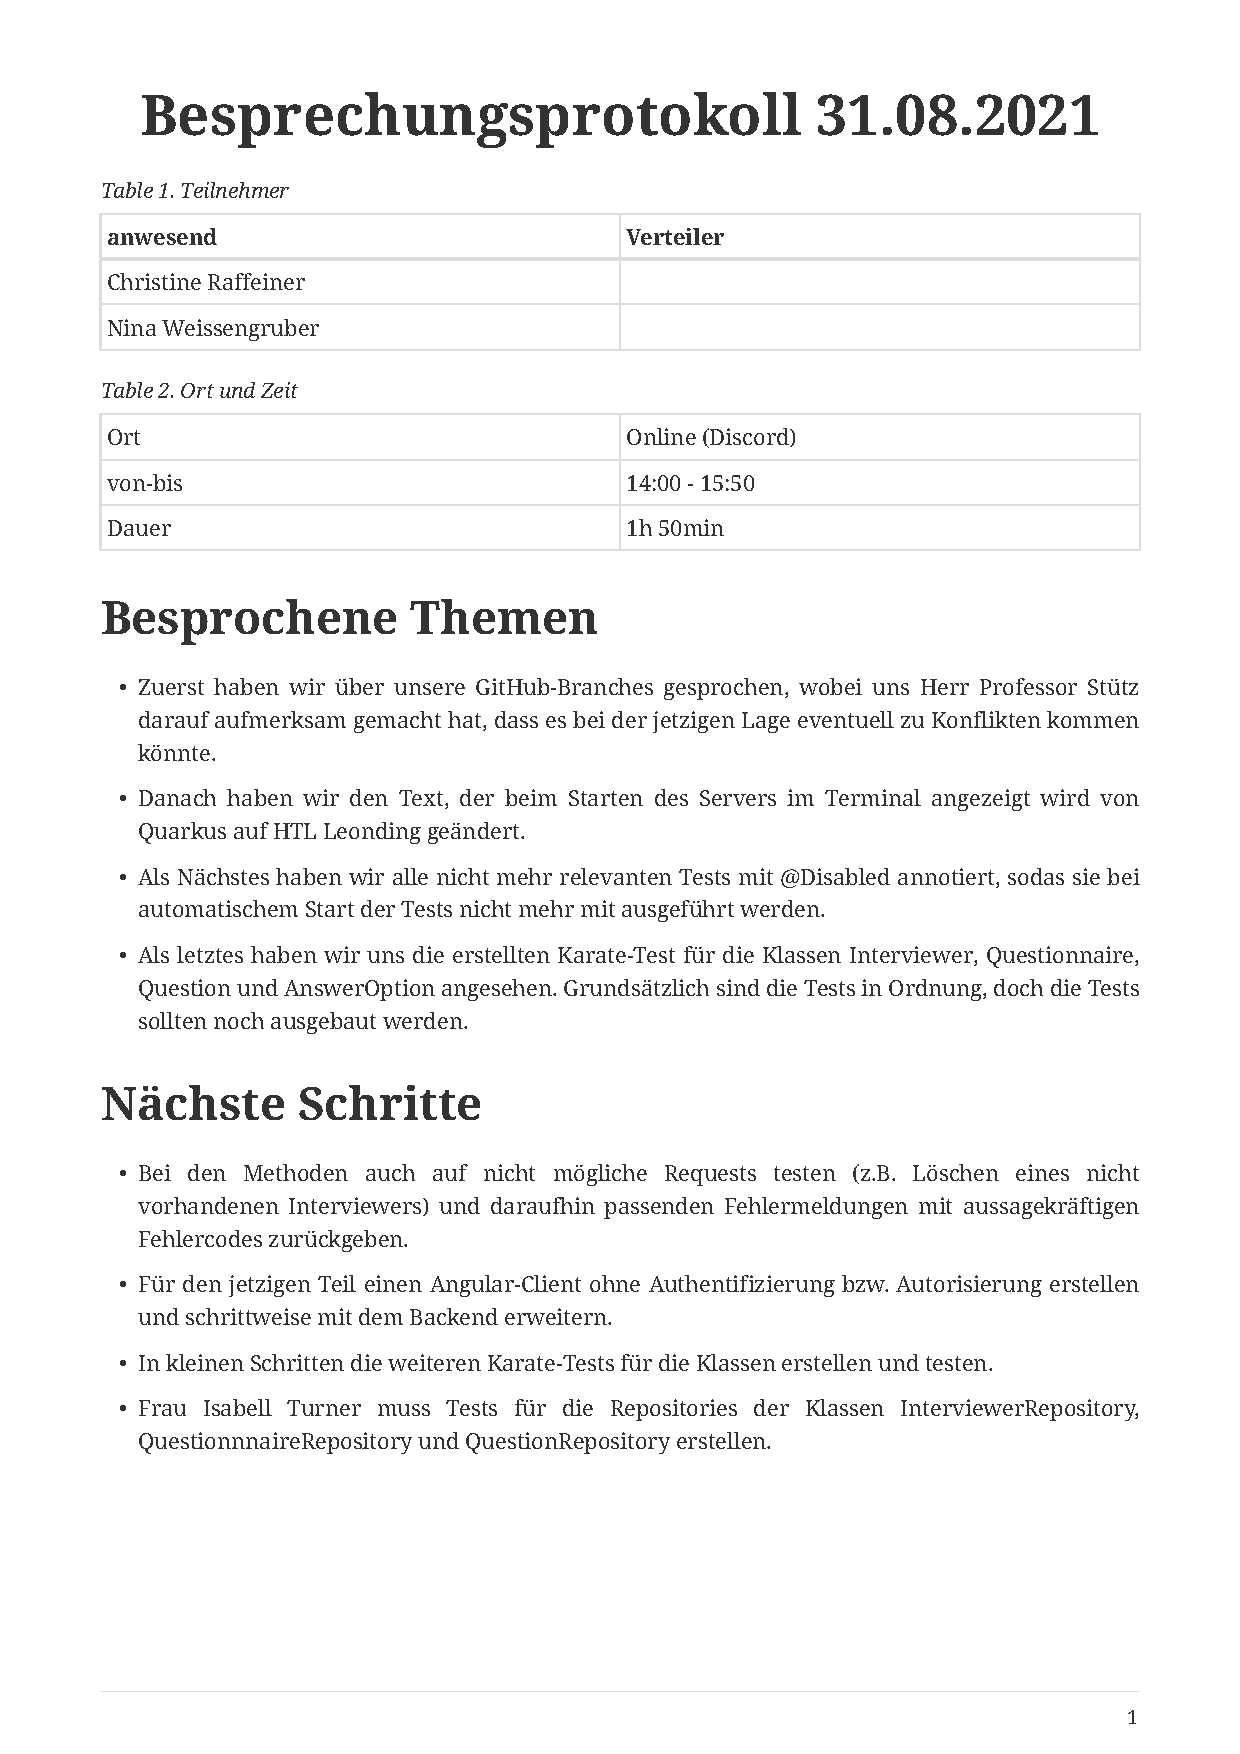
\includepdf{./protocols/meeting_31.08.2021}

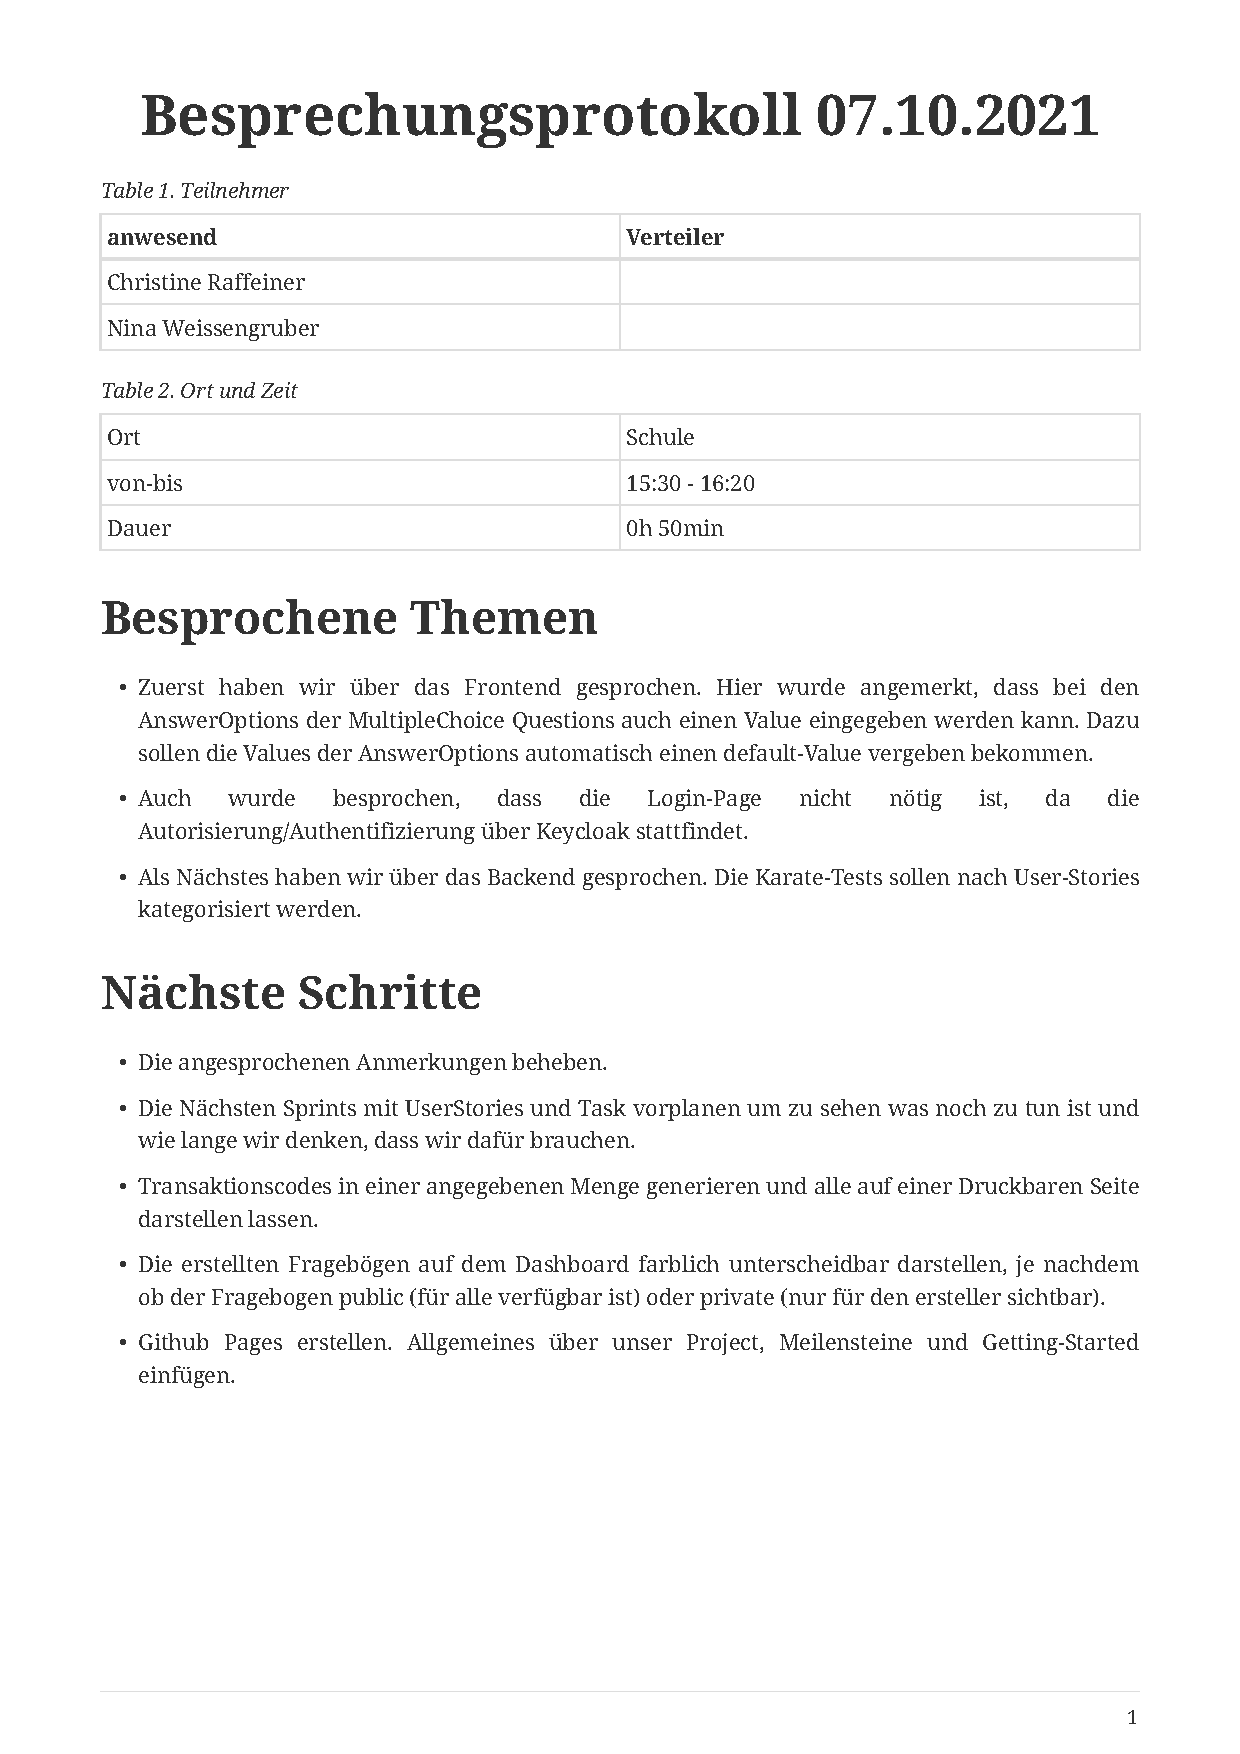
\includepdf{./protocols/meeting_07.10.2021}

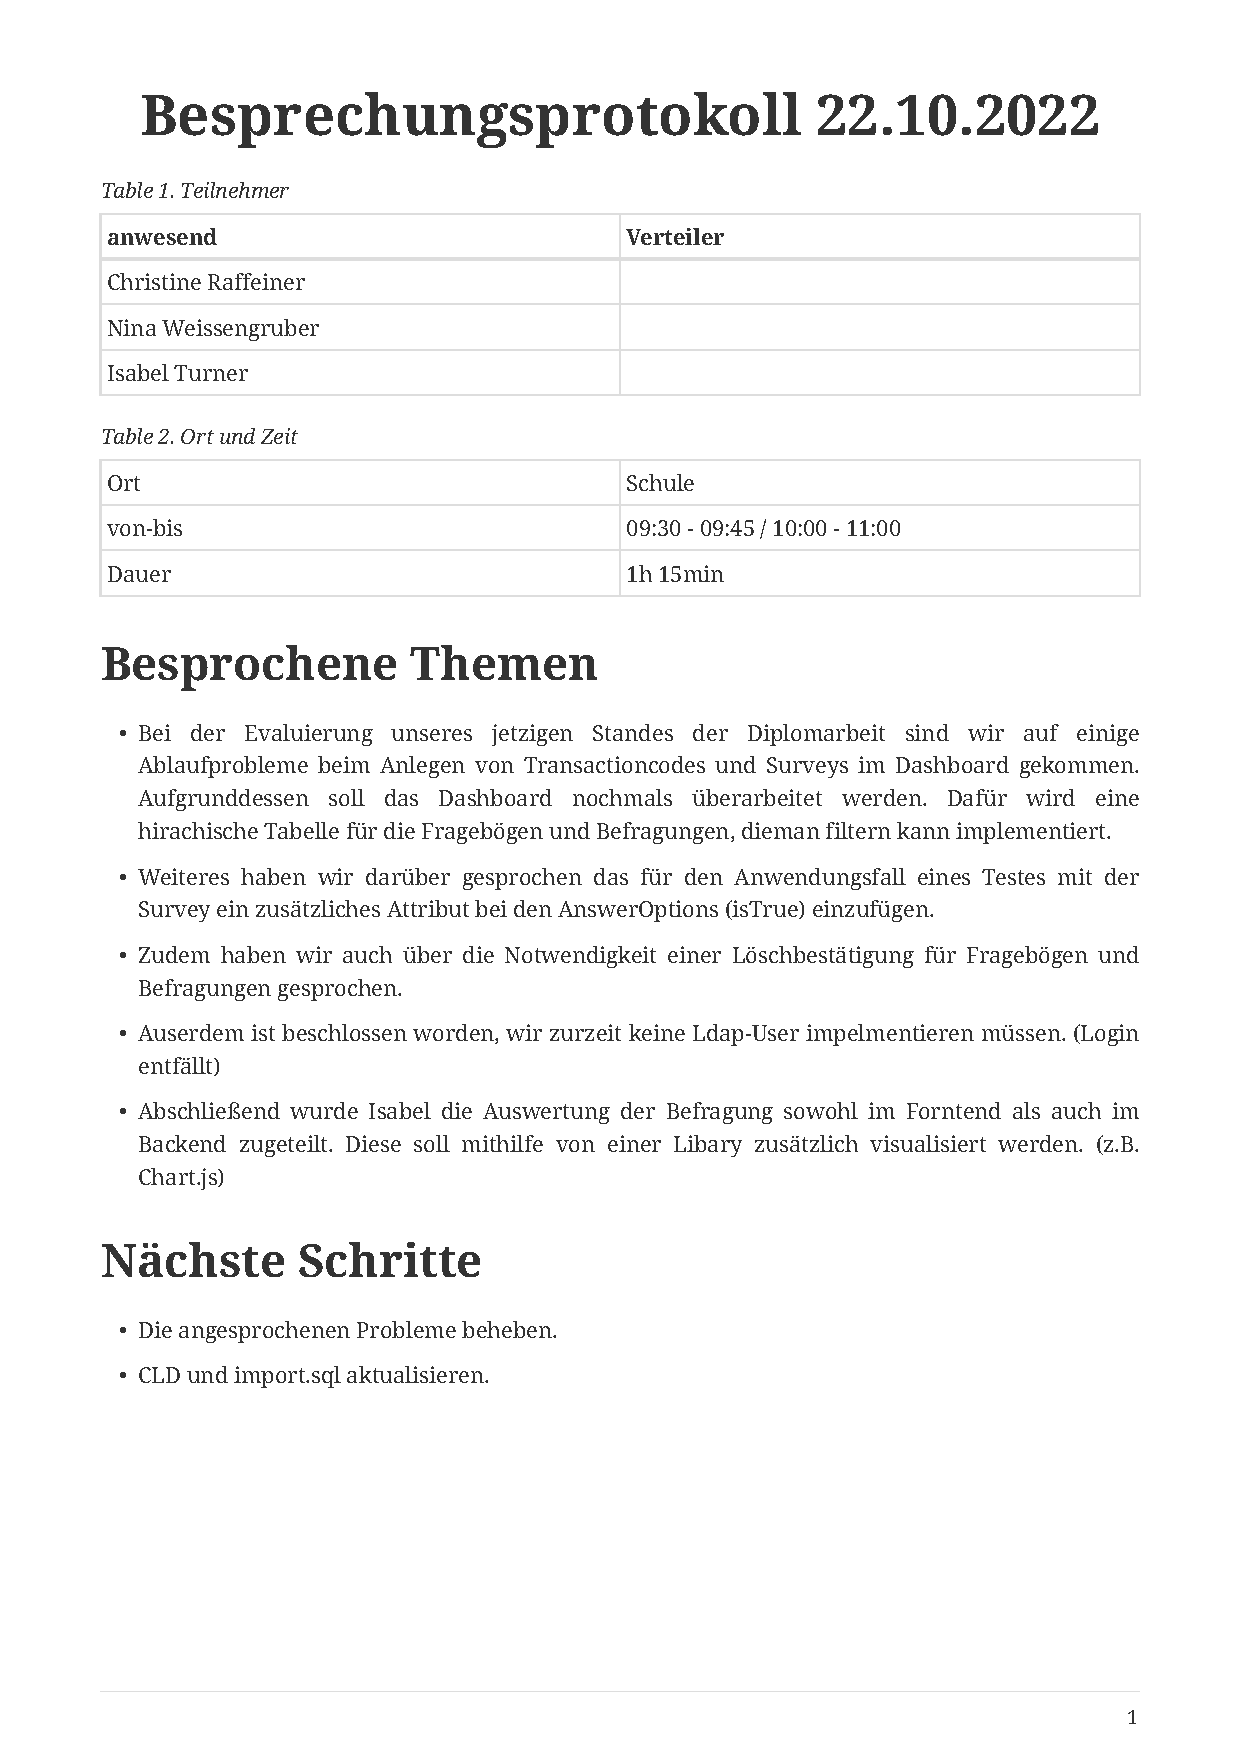
\includepdf{./protocols/meeting_22.10.2021}

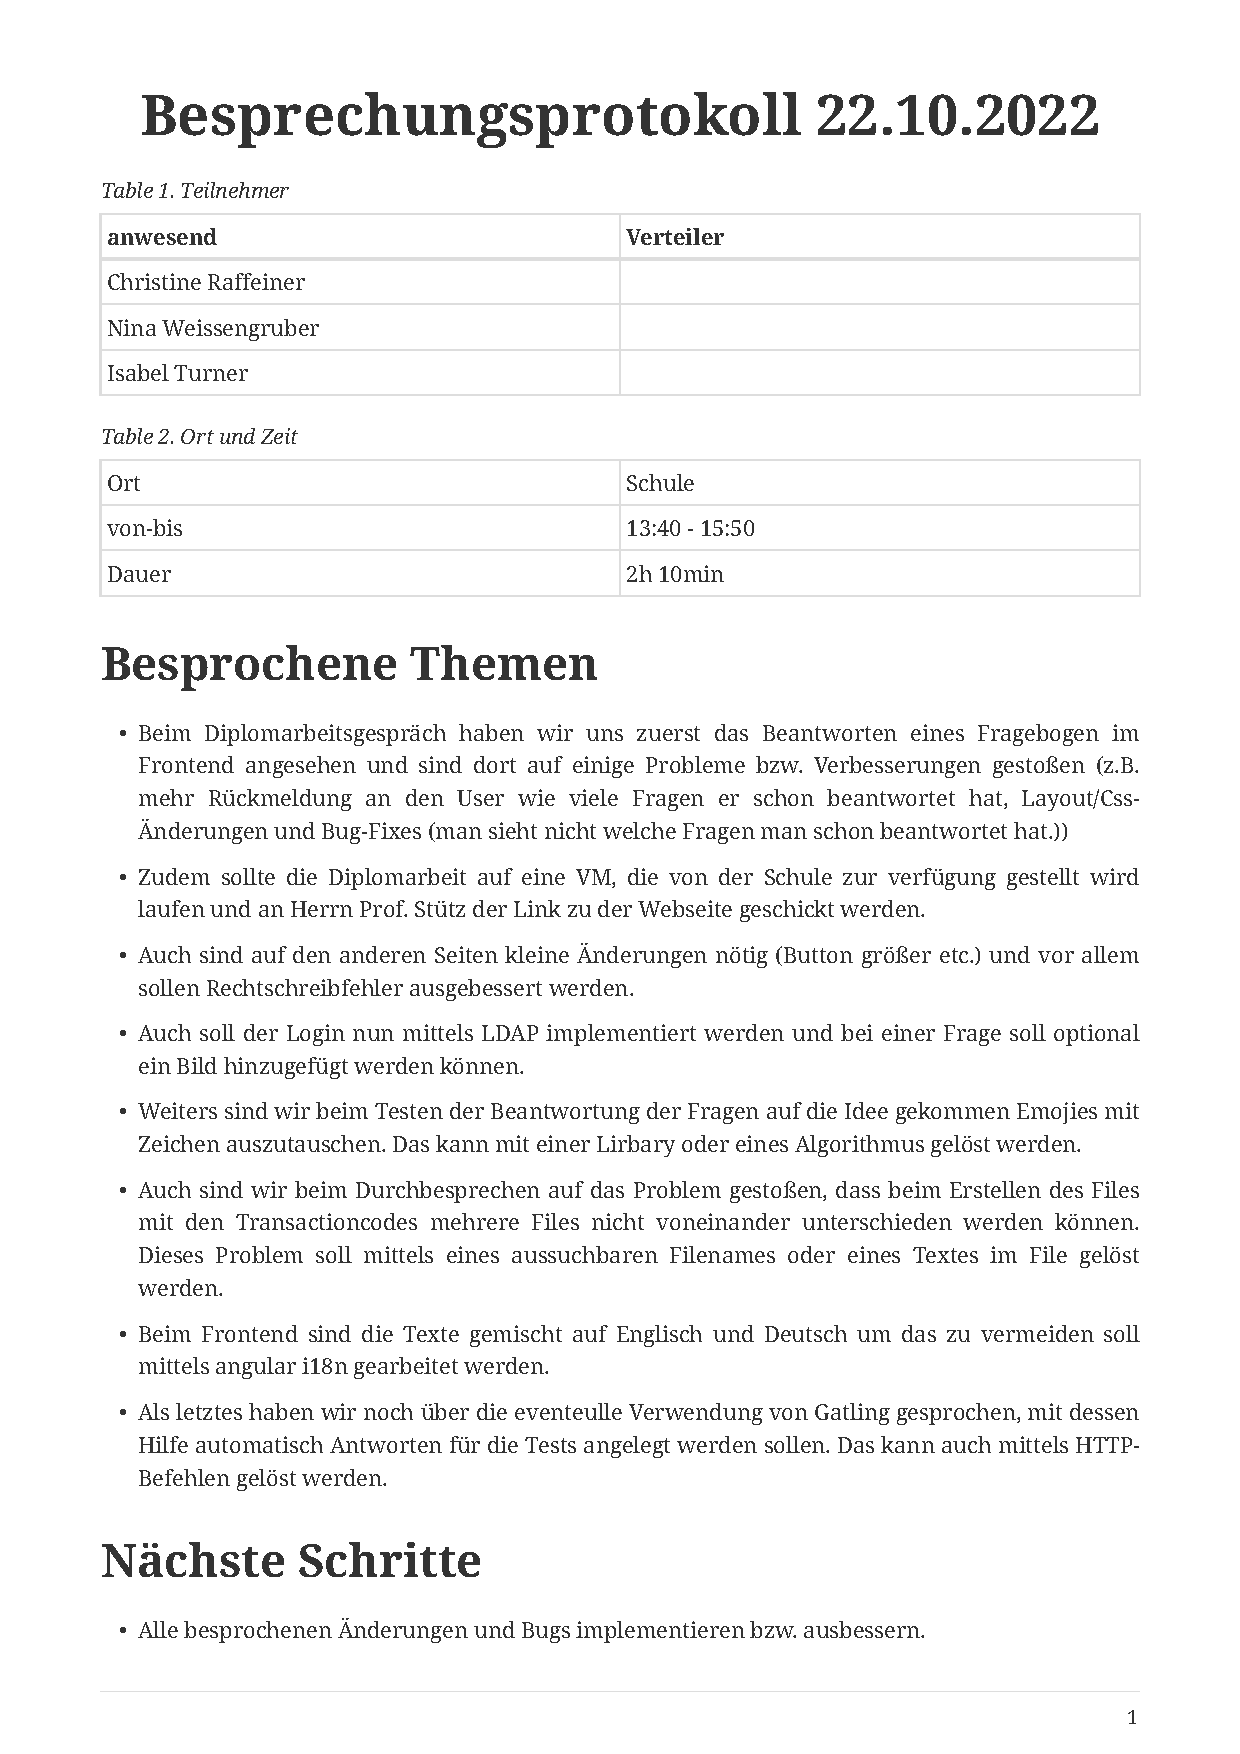
\includepdf{./protocols/meeting_21.01.2022}
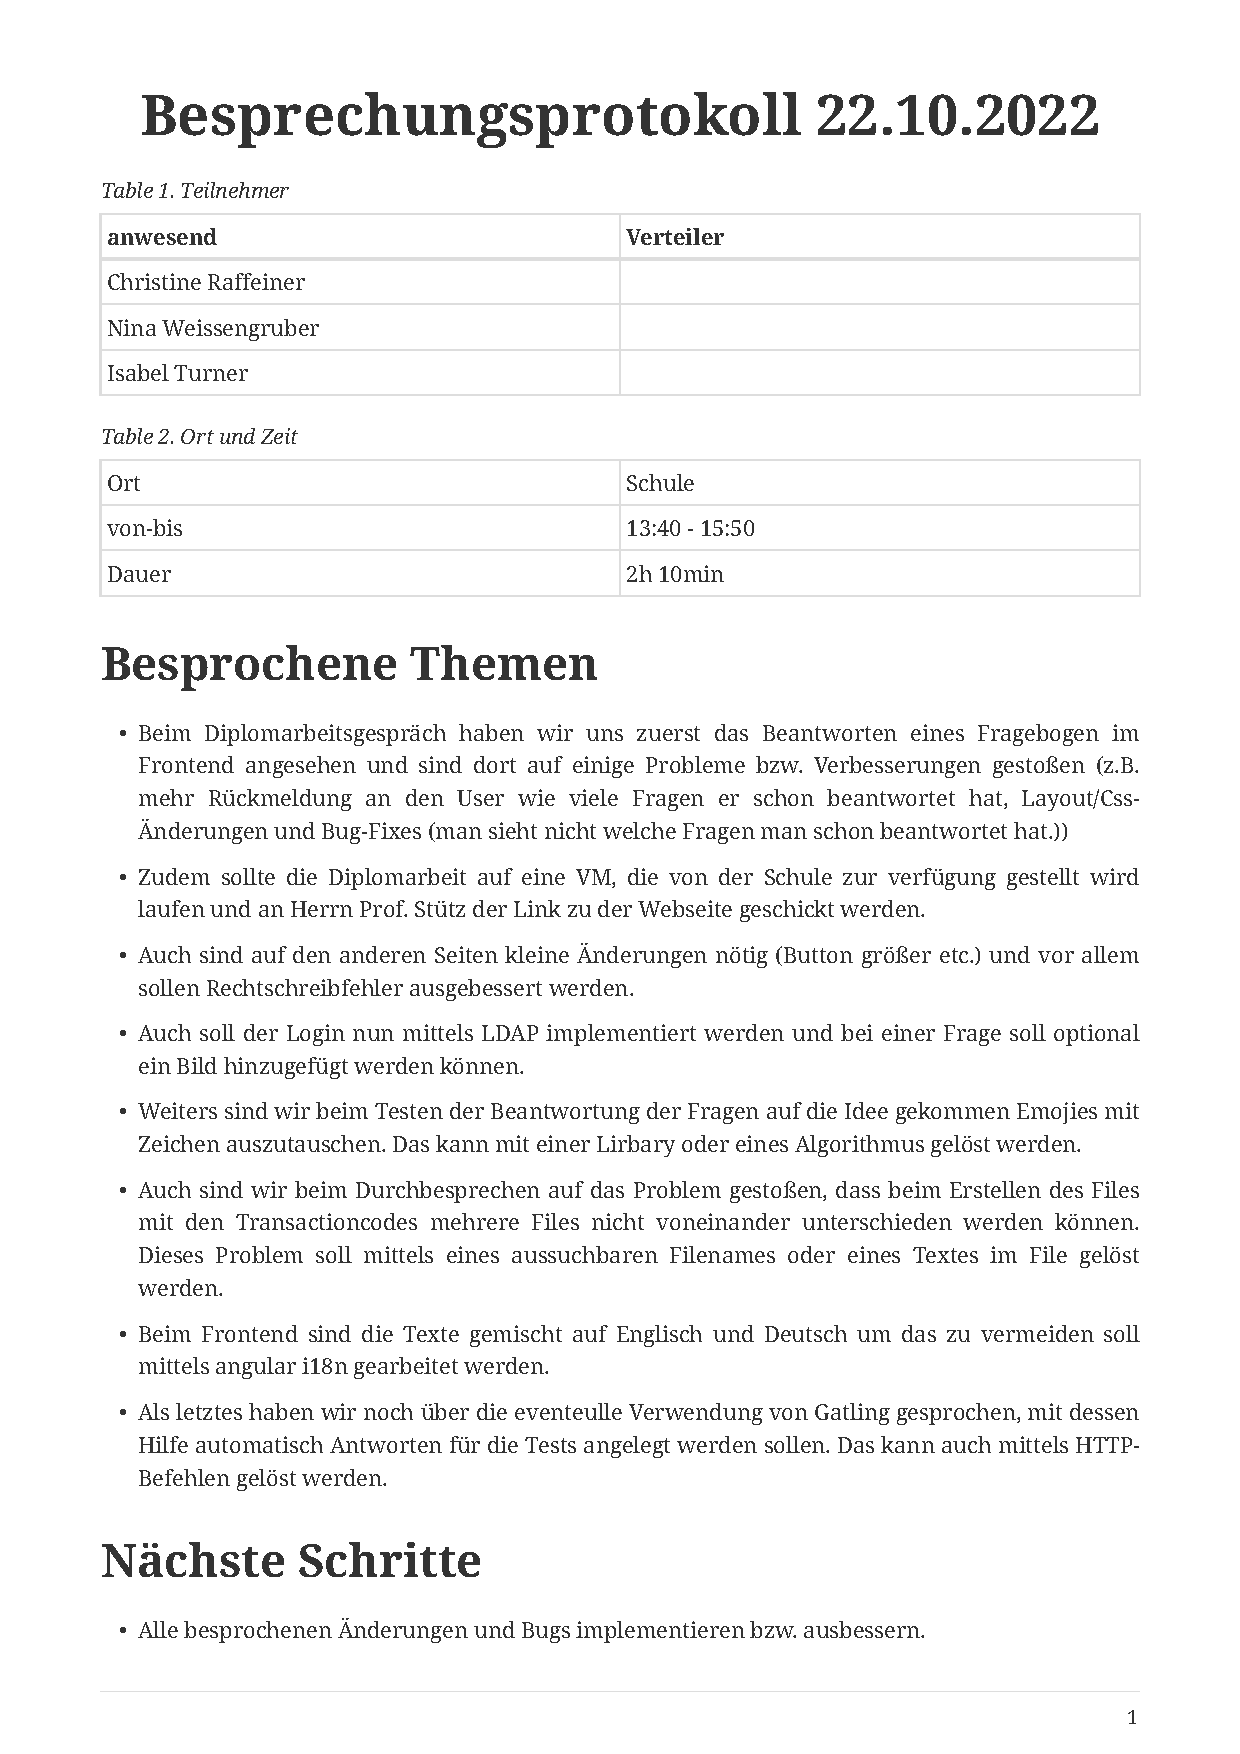
\includepdf[page=2]{./protocols/meeting_21.01.2022}

\chapter{Meilensteinliste und -analyse}
\label{meilensteile}
\setauthor{Raffeiner Christine}
Die erste Version der Meilensteinliste sah vor, dass die Arbeit innerhalb des Sommers,
während der Sommerferien implementiert und bis zu Schulbeginn fertiggestellt wird. 
\begin{table}[H]
    \centering
    \caption{Meilensteinliste Version 1}
    \label{tab:meilensteine1}
    \begin{tabular}{|c|l|}
        \hline
        05.07.2021 & Datenmodell fertiggestellt \\ \hline
        19.07.2021 & Backend (mit Endpoints) zum Ausfüllen eines vorhandenen Fragebogens erstellt \\ \hline
        02.08.2021 & Frontend zum Ausfüllen eines vorhandenen Fragebogens erstellt \\ \hline
        09.08.2021 & Backend (mit Endpoints) zum Erstellen eines Fragebogens erstellt \\ \hline
        23.08.2021 & Frontend zum Ausfüllen von Fragebögen erstellt \\ \hline
        13.09.2021 & Gesamtsystem mit Benutzerverwaltung und Docker-Deployment fertiggestellt \\ \hline
        \end{tabular}
\end{table}

Im Laufe des Sommers stellte sich bald heraus, dass diese Meilensteine aus vielerlei Gründen 
nicht eingehalten werden konnten. 
Die Meilensteine, (siehe Tabelle \ref{tab:meilensteine1}) (1) Datenmodell fertiggestellt und (2) Backend (mit Endpoints) 
die zum Ausfüllen eines vorhandenen Fragebogens erstellt, 
wurden in den Ferien verspätet fertiggestellt. Daraus folgend hat das Team die Meilensteine angepasst und eine neue
Liste erstellt (siehe Tabelle \ref{tab:meilensteine2}).

\begin{table}[H]
    \centering
    \caption{Meilensteinliste Version 2}
    \label{tab:meilensteine2}
    \begin{tabular}{|l|l|}
        \hline
        05.11.2021 & Backend und Frontend Funktionen zum Fragebogen erstellen fertiggestellt \\ \hline
        10.11.2021 & Frontend Dashboard fertiggestellt \\ \hline
        19.11.2021 & Backend und Frontend Funktionen zum Fragebogen ausfüllen fertiggestellt \\ \hline
        29.11.2021 & Backend zum Fragebogen ausfüllen fertiggestellt \\ \hline
        20.12.2021 & Backend und Frontend Login mittels Keycloak fertiggestellt \\ \hline
        10.01.2022 & Gesamtsystem Docker-Deployment fertiggestellt \\ \hline
    \end{tabular}
\end{table}

Die neue Meilensteinliste verschob die noch nicht erledigten Meilensteine nach hinten - mit dem Datum der 
Erreichung des letzten Meilensteines in den Winterferien. Das Team konnte auch  
diese Meilensteine nicht eingehalten. Da nun die Fertigstellung der Implementierung im Vordergrund 
stand wurden keine neuen Meilensteine mehr definiert und es wurde ohne Meilensteinliste auf die Fertigstellung hingearbeitet.
\newline
\newline
Schlussfolgernd ist zu sagen, dass die ursprünglichen Meilensteine oder zumindest die 2. Version der Liste, eingehalten hätten werden sollen.
Das Team ließ sich viel zu viel Zeit und war auch wenig konsequent mit der Einhaltung der gesetzten Ziele.
Zusätzlich wurde der gesamte Arbeitsumfang der Arbeit stark unterschätzt.

\chapter{Arbeitsverteilung}
\setauthor{Raffeiner Christine, Weissengruber Nina}
Die Arbeitsaufteilung war von Anfang an schnell und ohne Probleme entschieden. 
Die Programmierung des Backend und Testung fiel dabei Nina zu und Implementierung und Erstellung des Designs 
des Frontend wurde Christine überlassen. Außerdem wurde entschieden, dass Nina das Deployment übernimmt und 
Christine den Keycloak implementiert.

\subsection{Schriftliche Arbeitsteilung}
\begin{compactenum}
    \item Danksagung, Zusammenfassung und Inhaltsverzeichnis \big [ R \big ]
    \item Einleitung \big [ R \& W \big ]
    \item Ausgangssituation \big [ W \big ]
    \item Umfeldanalyse \big [ R \big ]
    \begin{compactenum}
        \item Vorgänger Projekte \big [ R \big ]
        \item Online Fragebogenwerkzeuge \big [ R \big ]
    \end{compactenum}
    \item Problembeschreibung \big [ W \big ]
    \item Aufgabenstellung \big [ W \big ]
    \item Ziele \big [ R \& W \big ]
    \item Systemarchitektur \big [ R \& W \big ]
    \item \begin{compactenum}
        \item Aktivitätsdiagramm \big [ W \big ]
        \item Klassendiagramm und Entity-Relationship-Modell \big [ R \big ]
    \end{compactenum}
    \item Technologien \big [ R \& W \big ]
    \begin{compactenum}
        \item Angular \big [ R \big ]
        \item Docker \big [ R \big ]
        \item Keycloak \big [ R \big ]
        \item Traefik \big [ R \big ]
        \item Oracle SQL-Developer \big [ R \big ]
        \item PlantUML \big [ R \big ]
        \item Markdown \big [ R \big ]
        \item Java \big [ W \big ]
        \item Quarkus \big [ W \big ]
        \item PostgreSql \big [ W \big ]
        \item Rest-API \big [ W \big ]
        \item Software Testing \big [ W \big ]
    \end{compactenum}
    \item Ausgewählte Aspekte \big [ R \& W \big ]
    \begin{compactenum}
        \item Besonders gut gelöste Programmteile \big [ R \& W \big ]
        \item Besondere Probleme die gelöst wurden \big [ R \& W \big ]
        \item Entwurfsentscheidung \big [ R \& W \big ]
    \end{compactenum}
    \item Implementierung \big [ W \big ]
    \item Projektorganisation \big [ R \big ]
    \begin{compactenum}
        \item Anforderungen \big [ R \big ]
        \item Mögliche Hilfsmittel \big [ R \big ]
        \item Problemlösung \big [ R \big ]
    \end{compactenum}
    \item ScreenDesign \big [ R \big ]
    \item \begin{compactenum}
        \item Handskizzen \big [ R \big ]
        \item ScreenDesign Prototyp \big [ R \big ]
    \end{compactenum}
    \item Ergebnis \big [ R \big ]
    \item \begin{compactenum}
        \item Zusammenfassung \big [ R \big ]
        \item Frontend \big [ R \big ]
    \end{compactenum}
    \item Resümee \big [ R \& W \big ]
    \item Anhang \big [ R \& W \big ]
    \begin{compactenum}
        \item Teamvorstellung \big [ R \& W \big ]
        \item Wichte Lektionen \big [ R \& W \big ]
        \item Protokolle \big [ R \big ]
        \item Meilensteinliste und -analyse \big [ R \big ]
        \item Arbeitsteilung \big [ R \& W \big ]
    \end{compactenum}
\end{compactenum}